\begin{myposter}{
    Глава 1. Уравнения движения и их свойства 
}

    \headerbox
    {Глава 1. Структура уравнений движения}
    {name=first,column=0,row=0,span=3}
    {
        {\huge\bf
            \vspace{10pt}
            \centering
            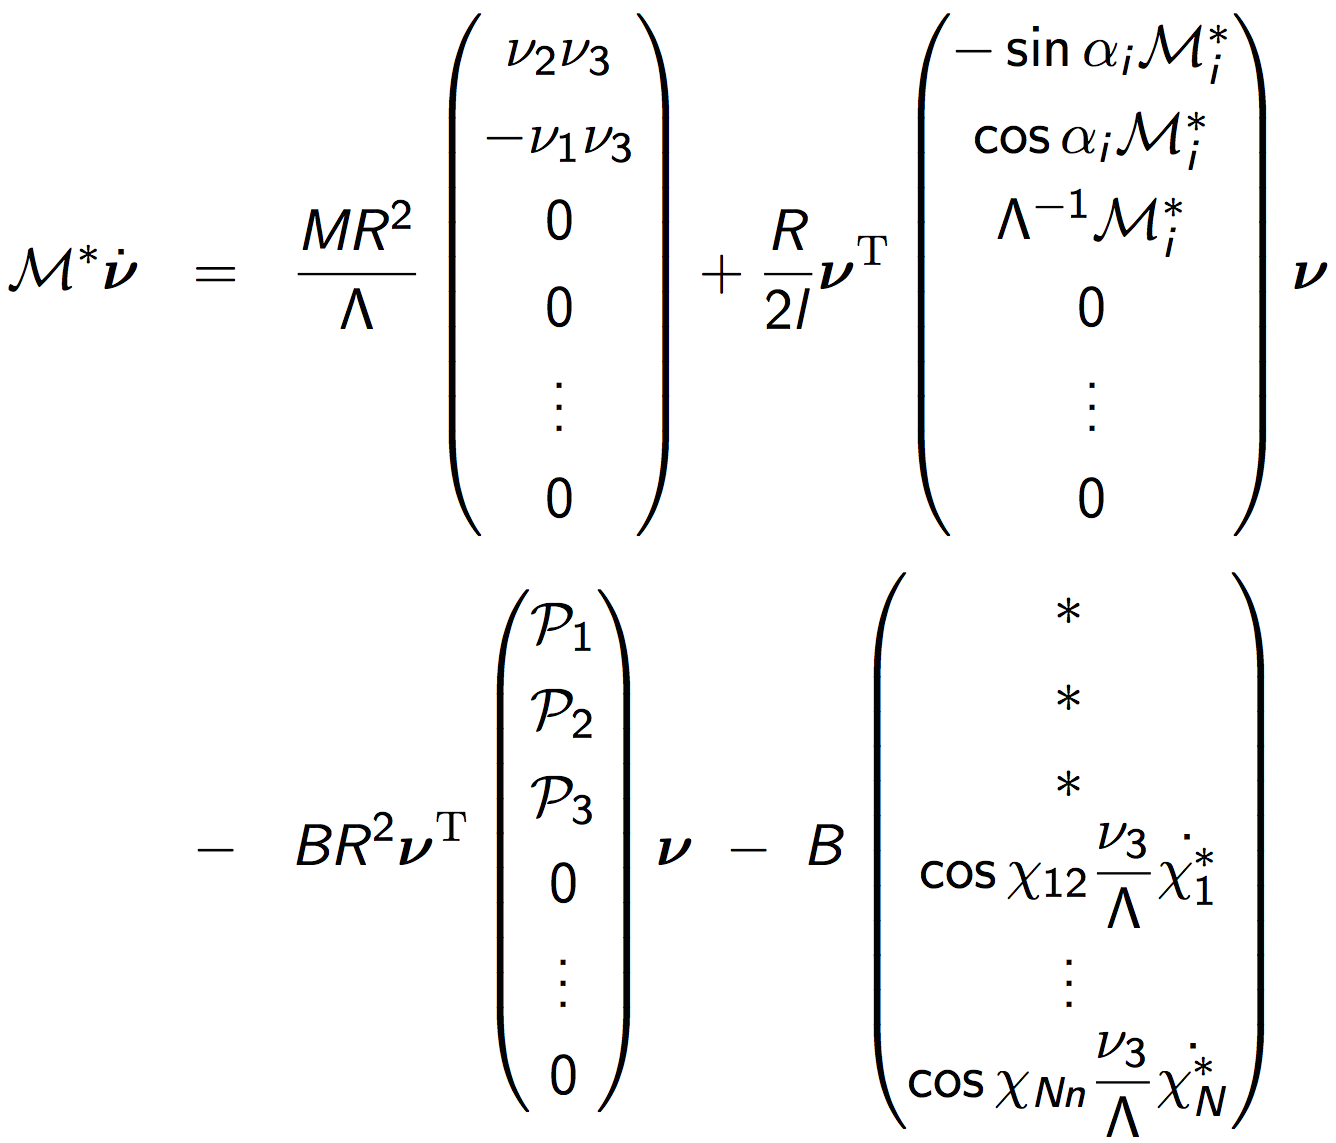
\includegraphics[width=0.7\textwidth]{content/pic/asypng/eq_struct.png}
            \vspace{10pt}
        }
    }
    
    \headerbox
    {Глава 1. Свойства уравнений движения}
    {name=second,column=0,row=1,below=first,span=3}
    {
        {\huge\bf
            \vspace{10pt}
            \begin{enumerate}
                \item При $B = 0$ уравнения движения совпадают с уравнениями безынерционной модели.
                \item Интеграл $m_{33}^*\nu_3 = \mathrm{const}$ разрушается при $B \neq 0$. \ $\dot{\nu_3} \textprop B$.
                \item Первые интегралы:
                $$\nu_s + \ddfrac{1}{\Lambda}\sin\chi_{ij}\nu_3 = const.$$
                \item Интеграл энергии \quad $\frac{1}{2}\vec{\nu}^\mathrm{T}\M^*(\chi_i)\vec{\nu} = h = \mathrm{const}$\\
                (связи автономны, идеальны, силы консервативны)
                \item $\nu_1 = \nu_2 = \nu_3 = 0 \quad \implies \quad \nu_s = \mathrm{const}$
                \item Замена псевдоскоростей $\vec{\nu} \rightarrow \lambda\vec{\nu}, \lambda \neq 0$ эквивалентна замене времени $t \rightarrow \lambda t$.
            \end{enumerate}
            \vspace{10pt}
        }
    }

\end{myposter}
